\subsubsection{Mother's Gestational Diabetes}
Gestational diabetes is a type of diabetes that occurs during pregnancy. It affects about 2-10\% of pregnant women and usually develops in the second or third trimester of pregnancy. Gestational diabetes can increase the risk of complications during pregnancy and delivery, as well as the risk of developing type 2 diabetes later in life.

The exact cause of gestational diabetes is not fully understood, but it is thought to be related to hormonal changes that occur during pregnancy. During pregnancy, the placenta produces hormones that can interfere with the body's ability to use insulin effectively. Insulin is a hormone that regulates blood sugar levels, and when the body is unable to use insulin properly, blood sugar levels can become elevated, leading to gestational diabetes.

Women who are at increased risk of developing gestational diabetes include those who are overweight or obese, have a family history of diabetes, have previously had gestational diabetes, have polycystic ovary syndrome (PCOS), or are older than 25 years of age.

Treatment for gestational diabetes usually involves dietary changes, such as reducing the intake of simple sugars and increasing the intake of complex carbohydrates, as well as regular exercise. In some cases, insulin injections may also be needed to control blood sugar levels. It is important for women with gestational diabetes to monitor their blood sugar levels regularly and attend all prenatal appointments to ensure that both they and their babies are healthy.

In \textbf{figure \ref{fig:gest_diabetes}} we can see a sudden spike in gestational diabetes among mothers in ACT.

\begin{figure}
  \centering
  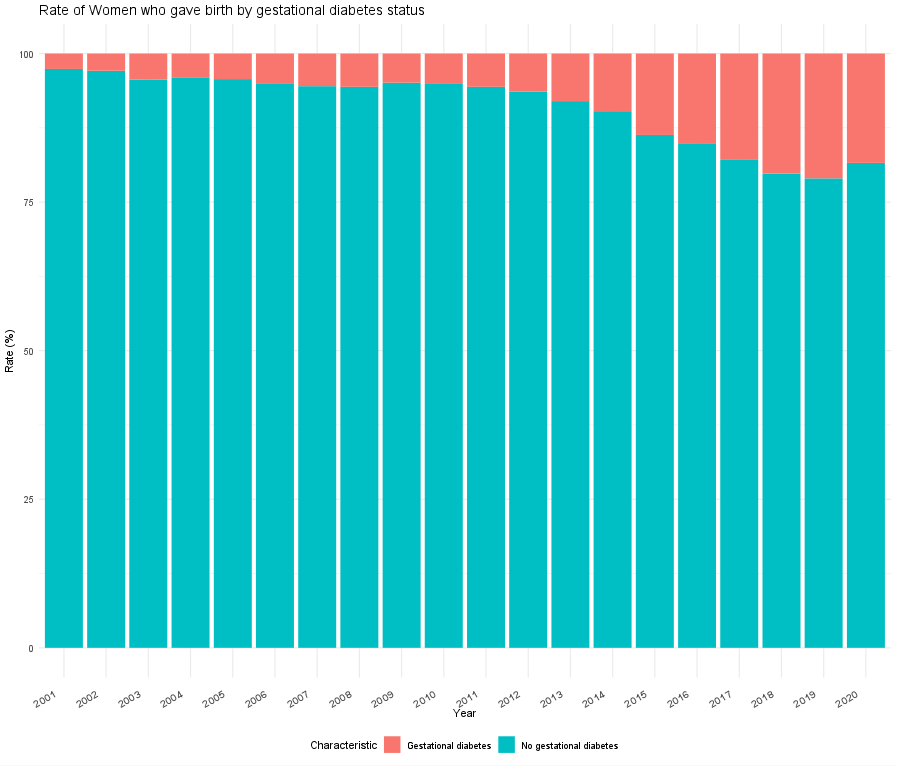
\includegraphics[width=0.90\textwidth]{subsections/baby_health/gestational_diabetes_rate.png}
  \caption{Gestational diabetes rate of mothers in ACT.}
  \label{fig:gest_diabetes}
\end{figure}